
\section{Parametry opisujące jakość powietrza}
\label{opis-parametrow}

Pomimo spadającej liczby śmierci spowodowanych niską jakością powietrza 
wewnętrznego, co sugeruje ogólną poprawę jakości powietrza, nie można 
stwierdzić wyeliminowania tego problemu. Na całym świecie aż 4\% wszystkich 
zgonów przypisuje się właśnie zanieczyszczeniom powietrza wewnętrznego. 
Szczególnie narażone są kraje biedne i mniej rozwinięte technologicznie \cite{owid}.

Pomijając tak drastyczne przypadki zła kondycja powietrza może powodować szereg mniej 
groźnych problemów zdrowotnych, takich jak pogorszenie zdolności rozwiązywania 
problemów i podejmowanie decyzji \cite{co2-effects}, co w szczególności dotyka placówki oświatowe i 
osoby tam przebywające. Bacząc na powyższe, oraz na fakt że człowiek średnio spędza większość dnia w swoim 
domu \cite{time-indoors}, nie licząc takich aktywności jak praca w zamkniętym pomieszczeniu, nowoczesne 
budynki powinny umożliwiać monitorowanie stanu powietrza wewnątrz 
ich w celu lepszej kontroli nad ich jakością.

Stan jakości powietrza wewnętrznego można opisać szeregiem parametrów: przepływ powietrza, 
pomiar stężenia cząsteczek stałych, tlenków węgla czy dwutlenku siarki. Jednymi z 
najczęściej stosowanych parametrów są jednak temperatura, wilgotność powietrza oraz 
zawartość dwutlenku węgla w powietrzu. 

\subsection{Temperatura}

Komfortowy przedział temperatur dla człowieka w zamkniętych pomieszczeniach w dużej 
mierze zależy od otaczającego klimatu i przyzwyczajeń z tego wynikających. Zależy on od takich czynników 
jak wiek, płeć, pora roku, klimat na danym obszarze czy rodzaj wykonywanej pracy.

W Polsce za minimalną dopuszczalną temperaturę w miejscu pracy przyjmuje się 18st. Celsjusza dla 
lekkiej pracy niewymagającej wysiłku fizycznego oraz 14st. dla pomieszczeń, w których wykonywane są prace 
fizyczne \cite{manutan-bhp}. Aktualne przepisy BHP nie normują jednak maksymalnej dopuszczalnej temperatury. 
Kolejnym dokumentem pomagającym przybliżyć komfortowy przedział temperatur w pomieszczeniach jest
"Rozporządzenie Min. Infrastruktury z 12.04.2002 w sprawie warunków technicznych jakim powinny odpowiadać 
budynki i ich usytuowanie", a dokładnie art. 134 punkt 2 \cite{rozp-bud}. Określono tam temperaturę na potrzeby obliczeń szczytowej 
mocy cieplnej w pomieszczeniach zależnie od ich przeznaczenia.
Dla przykładu, pomieszczenia przeznaczone na stały pobyt ludzi bez okryć zewnętrznych, nie wykonujących 
w sposób ciągły pracy fizycznej posiadają temperaturę obliczeniową 20st.C:

\begin{figure}[H]
    \caption{Fragment tabeli z Rozporządzenia przedstawiający temperatury obliczeniowe dla niektórych typów pomieszczeń}
    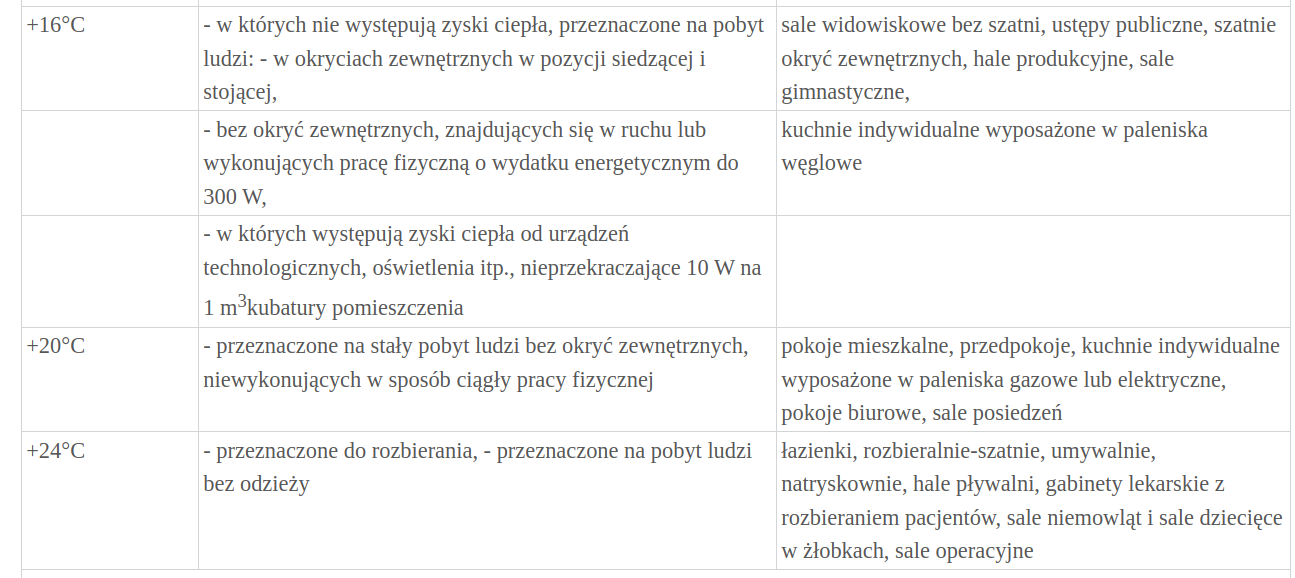
\includegraphics[width=\textwidth]{zdj/min-tabela.png}
\end{figure}

Za niska temperatura może powodować zwiększoną śmiertelność z powodu chorób układu oddechowego czy podwyższone 
ciśnienie \cite{who-cold}. Za wysoka zaś oprócz oczywistego dyskomfortu może doprowadzić zwiększonej śmiertelności, 
szczególnie u osób z chorobami układu oddechowego czy cierpiących na arytmię \cite{bmj-heat}.

W tej pracy za optymalny przedział temperatur przyjmuje się 18-22st. Celsjusza.

\subsection{Wilgotność}

Wilgotność powietrza można mierzyć na parę sposobów, natomiast odpowiednie aspekty tej pracy będą 
skupiały na wilgotności względnej - jest to stosunek wilgotności bezwzględnej powietrza do jej wartości 
maksymalnej w danej temperaturze \cite{termodynamika}

W pomieszczeniach biurowych o regulowanej temperaturze za optymalny zakres przyjmuje się 
od 25 do 60 \% wilgotności \cite{inz-bud}. Niższa wilgotność, szczególnie w połączeniu z niską temperaturą 
mogą przyczyniać się do zwiększonego występowania chorób układu oddechowego \cite{low-hum}. Za wysoka wilgotność 
zaś sprzyja rozwojowi i rozprzestrzenianiu się związków biologicznych (bakterie, wirusy, grzyby) 
powodujących alergie i choroby zakaźne \cite{high-hum}.

Podobnie jak temperatura, wilgotność zależy od wielu czynników i może zmieniać się bardzo dynamicznie, 
nawet w ciągu dnia. Wpływanie na wilgotność powietrza polega przede wszystkim na możliwości odczytu 
jego aktualnej lub historycznej wartości.

\begin{figure}[H]
    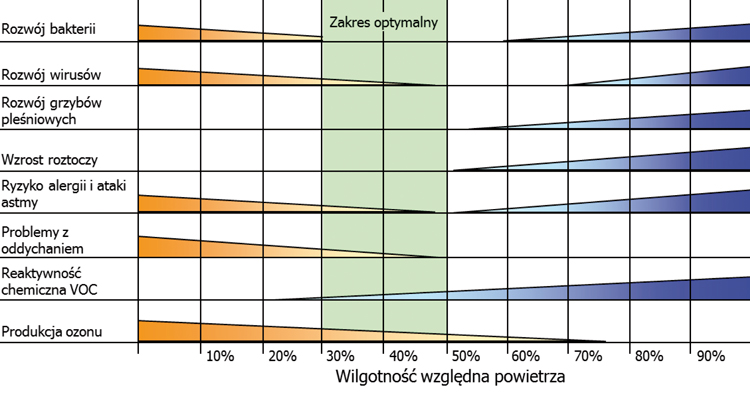
\includegraphics[width=\textwidth]{zdj/wilgotnosc_powietrza_w_pomieszczeniach.jpg}
    \caption{Wpływ wilgotności powietrza na nasilenie poszczególnych czynników}
\end{figure}

W związku z powyższym za optymalny przedział przyjmuje się od 30\% do 50\% wilgotności względnej 
powietrza.

\subsection{Dwutlenek węgla}

Podobnie jak w przypadku wilgotności, zawartość CO2 w powietrzu można mierzyć w wielu jednostkach. 
W tej pracy zdecydowano się jednak posługiwać się jednostką ppm - części na milion.

Za standard bezpiecznego poziomu CO2 w pomieszczeniu przyjmuje się wskaźnik Pettenkofera, który określa, 
że bezpieczne maksymalne stężenie tego związku w powietrzu wyrażone w częściach na milion wynosi 1000ppm \cite{pettenhofer}.

Rozporządzenie ministra rodziny, pracy i polityki społecznej z dnia 12 czerwca 2018 r. w sprawie 
najwyższych dopuszczalnych stężeń i natężeń czynników szkodliwych dla zdrowia w środowisku \cite{min-stezenia} pracy określa 
dopuszczalne stężenia szkodliwych dla człowieka substancji w trakcie pracy. Dla CO2 jest to:

* 9000 mg/m3 (~4,917ppm) - wartość średnia ważona, w ciągu 8-godzinnego dobowego i przeciętnego tygodniowo wymiaru pracy
* 27000 mg/m3 (~14,752ppm) - maksymalne stężenie, które może występować nie dłużej niż 15min, nie częściej niż 2 razy w ciągu zmiany i w odstępie dłuższym niż 1 godzina.

Standardowa ilość atmosferycznego dwutlenku węgla w powietrzu wynosi aktualnie około 417ppm. 
Liczba ta od początku Rewolucji Przemysłowej w 1750r. stale rośnie \cite{atmo-co2-change}, a według niektórych danych jest 
ono nawet 50\% wyższe niż sprzed wspomnianej daty \cite{50-percent}. Stężenie CO2 w powietrzu wyższe od 
wspomnianego wskaźnika Pettenkofera może powodować trudności w koncentracji, senność czy 
trudności z oddychaniem \cite{pettenhofer}.

\begin{figure}[H]
    \centering
    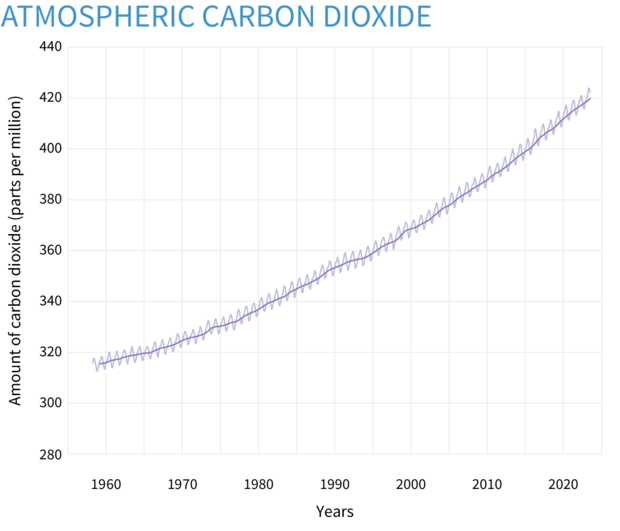
\includegraphics[width=0.8\textwidth]{zdj/more-co2.png}
    \caption{Wzrost stężenia dwutlenku węgla w atmosferze na przestrzeni lat}
\end{figure}

Za optymalny przedział wartości zawartości dwutlenku węgla w powietrzu przyjmuje się 400-1000ppm.